%\subsection{Tapered waveguide due to interface width} 
%tapered_width
The taper width affects the acceptable scale of the waveguide. The beam spot diameter at the working distance is about $1.5\mu$m, while the regular waveguide has smaller dimensions (w=$1\mu$m and h=$0.5\mu$m). In order to catch a complete view we discuss the tapered width starting with $1.2\mu$m to match the beam spot. Fig. \ref{fig:tapered_waveguide_wxx} presents the coupling behavior of the tapered waveguide along the variation of the interface width. From the figure it can be told that the coupling efficiency of this arrangement rise firstly with the width increasing and achieve its peak value at the width $d_{1}=2\mu$m and $2.2\mu$m. Then the efficiency falls as the interface width increasing. This tendency can be explained that a wider interface can confine more incident rays into the propagation tunnel but if the interface expands continually, other aspects, such as the divergence angle, may cause the decline of the coupling ability over the effect of the interface width.\\ 

\begin{figure}[!ht]
\centering
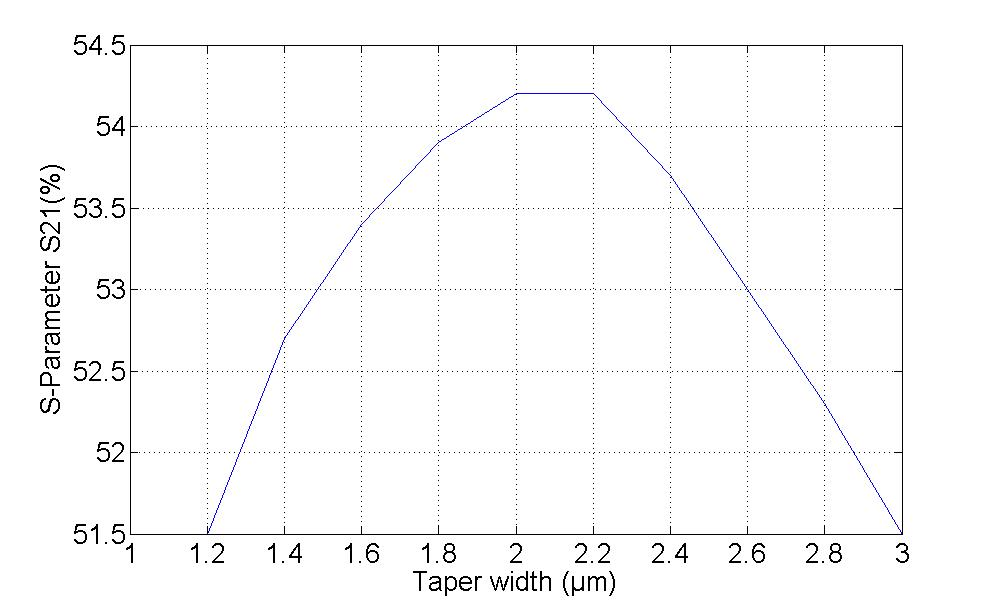
\includegraphics[width=0.7\textwidth]{bilder/tapered_waveguide_wxx}
\caption{Coupling efficiency between TLF and tapered waveguide with constant taper length $= 5.5\mu$m due to the variations of the interface width.}
\label{fig:tapered_waveguide_wxx}
\end{figure}
